% Reviewed text before the approved SPICE reorganisation. Not included in the paper.
\section{The NAUSICA concept}
\label{sec:nausica}

Reading the arriving ions (without amplification) requires exposed metal electrodes connected to charge-sensitive amplifiers (CSAs). Our proposed  \emph{Non-Amplified Ultra-Slow Ion CMOS ASIC} (NAUSICA) uses TopMetal CMOS technology~\cite{An2016TopmetalII} to implement this concept, following Refs.~\cite{Nygren_2018, mei2020topmetalcmosdirectcharge}. There is an important difference, however, with respect to these works, which attempted to design a system able to provide simultaneously good energy resolution and a good measurement of the track topology using ions. Alas, both requirements impose constraints that interfere with each other. Good energy resolution requires optimizing ion counting and minimizing noise. Good topological reconstruction demands pixels separated by a small pitch (e.g., of the order of diffusion, $\sim 2$ mm), which in turn multiplies the number of pixels and adds to the overall noise. The advantage of ITACA is that energy resolution is measured with excellent precision by electroluminescence, and thus the ion detector can prioritize the reconstruction of the topology. NAUSICA is designed with this goal in mind.

The principle of operation is as follows. The ions arrive at the metal pad over a time of order 1 second, taking a 10 cm extent along the drift direction as an extreme case. The resolution in $z$ should be of the order of the resolution in the transverse coordinates ($\sigma_z = 1-2$ mm). Since the drift velocity of the ions is $\sim 10$ cm/s, this translates into slicing the charge in buckets of $10-20$ ms, which implies a framed readout (about 50 frames of 20 ms each). The mean number of ions per pad in those buckets helps determine the feedback capacitance of the CSA.


\begin{figure}[!htbp]
    \centering
    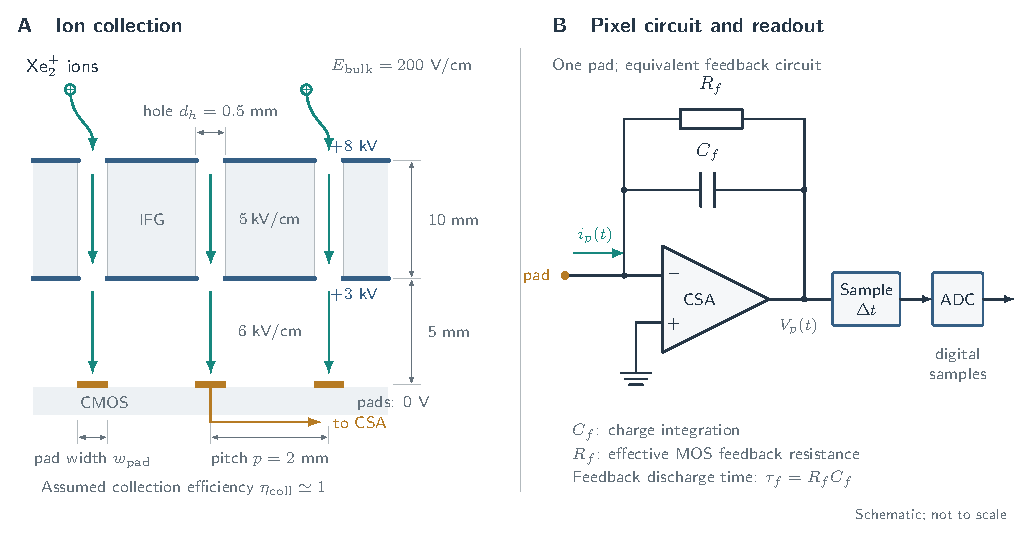
\includegraphics[width=\linewidth]{figures/nausica_concept.pdf}
    \caption{NAUSICA ion collection geometry (left) and equivalent pixel circuit (right). The drawing is schematic and not to scale.}
    \label{fig:nausicaa}
\end{figure}


\subsection{Charge collection and focusing}

The pad dimensions and pitch need to be chosen balancing the desired spatial resolution with the need for an acceptable signal-to-noise (S/N) per pad. Larger pads increase the collection but also the input capacitance, thus the need to focus the incoming ions in an area as small as possible. The left panel of Fig. \ref{fig:nausicaa} shows a schematic of the Ion Focusing Grid (IFG), which does this job.  We estimate the focusing requirement by comparing the electric flux through one pixel cell with that through its hole. Taking uniform fields in the drift region and inside the hole, full flux collection requires
\[
E_h\,\frac{\pi d_h^2}{4}\gtrsim E_{\rm bulk}p^2.
\]
Here $E_h$ and $E_{\rm bulk}$ are the fields inside the hole and in the drift region, respectively, $d_h$ is the hole diameter, and $p$ is the pixel pitch.
For a pitch of 2 mm, a bulk field of 200 V/cm and a hole field of 5 kV/cm, this gives a minimum hole diameter of approximately 0.45 mm. Thus, we take 0.5 mm as a preliminary design parameter. Full flux collection in this simple geometry implies a large ion collection efficiency that we take as one for the time being.


\subsection{Pixel electronics and readout}

The right panel of Fig. \ref{fig:nausicaa} shows a schematic of the electronics. Each pad is directly connected to the input of a CSA. The input current is integrated on a feedback capacitor $C_f$. A MOS transistor allows $C_f$ to discharge slowly. The gain is  $1/C_{f}$, and the signal decays with time constant $\tau_{f}$.


The sampled voltage includes charge accumulated in previous buckets. The charge arriving in each bucket is recovered from the change between successive samples, accounting for feedback discharge. Digitisation is performed at the periphery of the ASIC or on an external carrier, using one or a small number of multiplexed ADCs.

\subsection{Parameters of the design}

In summary, the pad size, pitch and active area must be chosen to sample and contain the ion track. The feedback capacitance and discharge time depend on the charge arriving at each pad and its distribution in time. The sampling interval, electronic noise and ADC range must allow the weaker parts of the track to be recorded while accommodating the largest signals.


\section{Signal formation and response of one pad}
\label{sec:single_ion}

Consider an ion, with charge $q=e$, arriving at a readout pad. The process of signal formation can be viewed in two steps:
\begin{enumerate}
\item As the ion approaches, a current is induced in the pad.
\item Then the CSA integrates it and produces the voltage sampled by the readout.
\end{enumerate}

Next, we describe each step:

\subsection{The induced current}

The weighting potential of a pad, $\phi_{w}(r)$, describes how an ion’s motion contributes to the signal on that pad. We calculate it for the detector geometry with the following boundary conditions: (a) the selected pad is held at unit potential and (b) all other electrodes at zero. Also the calculation is performed in the absence of charge.

We define positive current as current delivered into the CSA input by an approaching positive ion. With this convention, the meaning of $\phi_w$ follows from the Shockley--Ramo relation~\cite{riegler2016}
\begin{equation}
 \Delta Q=e\,\Delta\phi_w.
 \label{eq:single_charge}
\end{equation}

The current is the rate at which this signal develops:
\begin{equation}
 i_1(t)=e\frac{\dd\phi_w(\mathbf r(t))}{\dd t}.
 \label{eq:single_ramo}
\end{equation}
Near a small pad, $\phi_w$ changes rapidly with position, so most of the signal is induced during the final approach.

For the analytical calculation we use a square pad of side $2a$, embedded in an infinite grounded plane. The gas occupies a homogeneous half-space above the plane. The ion approaches the centre of the pad along its normal at constant speed $v$. The gap width $g$ is the distance between the lower IFG electrode and the pad plane. This geometry provides a simple pad response. In this simple approximation, the IFG and the dielectric structure of the CMOS surface are not included in its weighting potential. Appendix~\ref{app:single_ion} gives the derivation and boundary conditions.

Place the pad at $z=0$ and take collection to occur at $t=0$, so that $z=-vt$ before collection. The weighting field on the central axis is
%
\begin{equation}
 W(z)=-\frac{\dd\phi_w}{\dd z}
 =\frac{4a^2}{\pi(z^2+a^2)\sqrt{z^2+2a^2}}.
 \label{eq:single_weight}
\end{equation}
%
For an ion entering this gap at $z=g$ and $t_g=-g/v$, the current is
%
\begin{equation}
 i_1(t)=
 \begin{cases}
 evW(-vt),&t_g\leq t<0,\\
 0,&\text{otherwise}.
 \end{cases}
 \label{eq:single_current}
\end{equation}
%
Its integral over this finite trajectory is $Q_g=e[1-\phi_w(g)]$.

\subsection{Signal size and duration}

As a numerical example, we take the parameters shown in the left panel of Fig. \ref{fig:nausicaa}: a pad of side \SI{\SignalPadWidth}{mm} and a gap of \SI{\SignalGap}{mm}. We estimate the gap velocity from $v=\mu E_g$, using the mobility inferred from the bulk drift speed and assuming it remains constant in the gap. With $E_g=\SI{\SignalGapField}{kV/cm}$, this gives $v=\SI{\GapSpeed}{m/s}$.

The current rises as the ion approaches the pad and reaches
\begin{equation}
 i_1(0^-)=\frac{2\sqrt{2}}{\pi}\frac{ev}{a}
 =\SI{\PeakCurrent}{fA}.
 \label{eq:single_peak}
\end{equation}
%
Most of the signal is induced close to the pad (Figure~\ref{fig:single_ion_current}). The final $\sim$\SI{200}{\micro\second} before collection contain 90\% of the full-path charge $e$ \footnote{Here ``full path'' means extending the same analytical trajectory to infinite distance.}. For the finite gap used in the calculation (Appendix~\ref{app:single_duration}),
%
\begin{equation}
 Q_g=e[1-\phi_w(g)]=\GapChargeFraction\,e.
 \label{eq:single_gap_charge}
\end{equation}
%

\begin{figure}[!htbp]
 \centering
 \includegraphics[width=\linewidth]{single_ion_current.pdf}
 \caption{Single-ion current across the full gap (left) and during the final approach (right), for the square-pad model described above. The upper axes show the time remaining before collection. The shaded region contributes 90\% of the full-path charge.}
 \label{fig:single_ion_current}
\end{figure}

\subsection{The CSA voltage}

We describe the CSA by an ideal amplifier with feedback capacitance $C_f$ and an effective resistance $R_f$ representing the MOS discharge path. The output voltage $V_1$ is measured relative to its baseline. The input current is shared between the feedback capacitor and the discharge path:
\begin{equation}
 i_1(t)=-C_f\frac{\dd V_1}{\dd t}-\frac{V_1}{R_f}.
 \label{eq:csa_current_balance}
\end{equation}
Where rhe first term describes charge integration and the second feedback discharge. With the discharge time $\tau_f=R_fC_f$, this becomes
%
\begin{equation}
 \frac{\dd V_1}{\dd t}+\frac{V_1}{\tau_f}
 =-\frac{i_1(t)}{C_f}.
 \label{eq:csa_ode}
\end{equation}
%
Setting $V_1(t_g)=0$, we find the solution
\begin{equation}
 V_1(t)=-\frac{1}{C_f}\int_{t_g}^{t}
 i_1(t')\exp\left[-\frac{t-t'}{\tau_f}\right]\dd t'.
 \label{eq:csa_solution}
\end{equation}
With this convention positive input current produces a negative voltage. Once collection is complete, the voltage decays exponentially, $V_1(t)=V_1(0)\exp(-t/\tau_f)$.

If discharge is negligible during the pulse, the voltage at collection is $V_1(0)=-Q_g/C_f$. Taking an  illustrative value of $C_f=\SI{\ReadoutCapacitance}{fF}$, the resulting voltage is \SI{\SingleIonIdealVoltage}{\micro\volt}. Figure~\ref{fig:single_ion_response} and Table~\ref{tab:single_ion_response} shows the idealized response of the CSA ---not including substantial effects such as linear response; transistor noise, finite amplifier bandwidth and saturation---

\begin{figure}[!htbp]
 \centering
 \includegraphics[width=\linewidth]{single_ion_response.pdf}
 \caption{CSA voltage magnitude for the finite-gap current in Figure~\ref{fig:single_ion_current}, with collection at $t=0$. The CSA has $C_f=\SI{\ReadoutCapacitance}{fF}$ and linear feedback, with the discharge times shown in the legend.}
 \label{fig:single_ion_response}
\end{figure}

\begin{table}[!htbp]
 \centering
 \begin{tabular}{rrr}
\toprule
$\tau_f$ (ms) & Peak $|V_1|$ ($\mu$V) & Fraction of $Q_g/C_f$ (\%) \\
\midrule
0.03 & 14.46 & 27.11 \\
1 & 49.12 & 92.12 \\
10 & 52.86 & 99.13 \\
$\infty$ & 53.32 & 100.00 \\
\bottomrule
\end{tabular}

 \caption{Peak response to the finite-gap single-ion current in Figure~\ref{fig:single_ion_current}. The last column compares the peak magnitude with the ideal-integrator value $Q_g/C_f$.}
 \label{tab:single_ion_response}
\end{table}

The induced current when several ions arrive during a readout frame is the sum of the individual ion-induced currents. For ions following the same final trajectory and collected on the same pad at times $t_k$, the linear model gives
\begin{equation}
 i_p(t)=\sum_k i_1(t-t_k),\qquad
 V_p(t)=\sum_k V_1(t-t_k).
 \label{eq:pad_superposition}
\end{equation}

%% Draft for author review. New material; preceding reviewed prose is unchanged.
\section{Beyond the ideal CSA model}
\label{sec:realistic_csa}

The ideal CSA keeps its input at a fixed potential and responds without delay. A real amplifier has finite gain and bandwidth. Some of the incoming charge can therefore remain on the input capacitance, and the output takes time to develop. Electronic noise also limits the charge that can be resolved. We extend the model to include these effects, using the circuit proposed by Rogelio as a starting point. The calculation describes small signals about a fixed operating point; the transistor circuit must establish the range over which this approximation holds.

\subsection{Finite gain and response time}

Let $C_{\rm in}$ be the capacitance between the input node and ground, including the pad, amplifier input and stray capacitances, but excluding $C_f$. We represent the amplifier by an open-loop gain
\begin{equation}
 A(s)=\frac{A_0}{1+s/\omega_a},\qquad V(s)=-A(s)V_{\rm in}(s),
 \label{eq:realistic_gain}
\end{equation}
where $s$ is the Laplace variable, $A_0$ is the DC gain and $\omega_a$ is the angular frequency of the amplifier pole. The feedback elements remain $C_f$ and an effective resistance $R_f$. Balancing the input current gives the current-to-voltage response
\begin{equation}
 H_I(s)\equiv\frac{V(s)}{I(s)}
 =-\frac{A(s)}{sC_{\rm in}+[1+A(s)](R_f^{-1}+sC_f)}.
 \label{eq:realistic_transimpedance}
\end{equation}
Appendix~\ref{app:realistic_csa} gives the derivation and its time-domain form.

The effect of finite gain is particularly simple when the amplifier has settled but feedback discharge is still negligible. For an injected charge $Q$, a frequency-independent gain $A_0$ gives
\begin{equation}
 V=-\frac{Q}{C_f+(C_{\rm in}+C_f)/A_0}.
 \label{eq:realistic_charge_gain}
\end{equation}
The ideal value $-Q/C_f$ is approached when $A_0C_f\gg C_{\rm in}+C_f$. Thus reducing $C_f$ increases the ideal gain, but also makes the amplifier gain requirement more demanding. This reduction in voltage is an electrical effect; it does not imply that fewer ions reach the pad. Equation~\eqref{eq:realistic_transimpedance} also accounts for the finite response time. The ideal approximation requires sufficient gain throughout the frequencies that contribute to the signal.

\subsection{Several ions in a readout frame}

For $k$ ions collected at times $t_j$, the input is the sum of the finite-gap currents calculated in Section~\ref{sec:single_ion}:
\begin{equation}
 i_k(t)=\sum_{j=1}^{k}i_1(t-t_j),\qquad
 V_k(t)=\int_{-\infty}^{t}h_I(t-t')i_k(t')\dd t',
 \label{eq:realistic_packet}
\end{equation}
where $h_I$ is the impulse response corresponding to $H_I$. Each ion contributes an integrated input charge $Q_g$. We first consider simultaneous arrivals and arrivals spread uniformly over a frame of duration $\Delta t$. These are controlled examples for comparing circuit responses; the arrival distributions from tracks are considered in the following section.

The current can begin before the frame in which an ion is collected, and the voltage can persist into later frames. We therefore retain the circuit state across frame boundaries and compare the sampled response with the charge actually induced during each frame. An additional packet in the preceding frame tests the effect of this retained signal.

For comparison with the ideal model, we estimate the frame charge from two consecutive samples using
\begin{equation}
 \widehat Q_n=-K\left(\overline V_n-\alpha\overline V_{n-1}\right),\qquad
 \alpha=e^{-\Delta t/\tau_f},\qquad
 K=C_f\frac{\Delta t/\tau_f}{1-\alpha},
 \label{eq:realistic_estimator}
\end{equation}
with $\tau_f=R_fC_f$. Here $\overline V_n$ denotes the measured sample, including any averaging during its acquisition. For instantaneous samples, Eq.~\eqref{eq:realistic_estimator} is exact for an ideal CSA driven by constant current within the frame, as shown in Appendix~\ref{app:single_ion}. With finite amplifier response or a different arrival history it is an estimator whose bias must be calculated. We compare it with $Q_n=\int_{t_{n-1}}^{t_n}i_k(t)\dd t$ rather than assuming that every collected ion contributes its full signal within the same frame.

\subsection{Noise in the recovered charge}

We describe the amplifier noise by an equivalent input voltage source and an input current source, assumed independent. Their spectra include white and flicker voltage noise, and current noise from the input and feedback path~\cite{tiNoise2007,spielerNoise1998}. The same circuit response used for the signal propagates these sources to the output. The sampling aperture and frequency limits are specified as part of the noise calculation. An effective MOS discharge resistance alone is insufficient to determine the noise of that transistor.

Let $C_V(0)$ be the variance of a voltage sample and $C_V(\Delta t)$ the covariance of consecutive samples. The variance of the estimated charge is
\begin{equation}
 \sigma_{\widehat Q}^{2}
 =K^2\left[(1+\alpha^2)C_V(0)-2\alpha C_V(\Delta t)\right].
 \label{eq:realistic_noise_charge}
\end{equation}
The covariance term matters because consecutive samples contain noise from the same circuit. Appendix~\ref{app:realistic_noise} derives these quantities from the noise spectra.

The ratio $\sigma_{\widehat Q}/e$ expresses the estimator noise in elementary-charge units. To infer sensitivity to ions, we also need the response to the specified arrival distribution. If $g_n$ is the mean estimated charge per ion for that distribution and sampling phase, then
\begin{equation}
 {\rm S/N}_n(k)=\frac{k|g_n|}{\sigma_{\widehat Q}},\qquad
 k_{\min,n}=\frac{\rho\,\sigma_{\widehat Q}}{|g_n|},
 \label{eq:realistic_sensitivity}
\end{equation}
where $\rho$ is the required signal-to-noise ratio. This is a conditional sensitivity for the chosen input and electronics parameters. Fluctuations in ion arrivals and the performance of a threshold applied across many pads require a separate calculation.

\subsection{Comparison with a circuit calculation}

The model defines quantities that can be compared directly with a SPICE calculation: input current, output waveform, charge recovered at the sampling times and noise in that charge estimate. The supplied inputs include the single-ion current, simultaneous and distributed arrivals, and a previous-frame packet. Their timing and integrated charge are fixed before changing the circuit. Rogelio's transistor calculation can then determine the attainable gain, bandwidth, discharge behaviour and noise, and test where the linear approximation fails. These results will replace the illustrative circuit parameters when the device model is available.

% Numerical results will be inserted after implementation and independent review.
% The operational handoff is tracked separately in readout/specs_to_spice.md.


\section{Beyond the ideal CSA model}
\label{sec:realistic_csa}

The next step is to make our model more realistic. The ideal CSA described in the previous section keeps its input at a fixed potential and responds immediately to an input charge.  Instead, a real amplifier has finite gain and a finite bandwidth. This has two implications. With finite gain, the input voltage is no longer fixed, and the output signal is smaller than the ideal value $Q/C_{f}$. Finite bandwidth limits how quickly the output can respond to the arriving current. Electronic noise also sets a limit on the minimum charge that can be measured. In this section, we extend the model to include these effects. The more realistic CSA model also includes the capacitance of the pad and amplifier input. The feedback circuit consists of a capacitor and a MOS discharge path, represented here by an effective resistance. Our improved model, however, still assumes a linear response. The range of validity of this assumption will be established by our last step, using  SPICE simulations.


\subsection{Finite gain and response time}

\begin{figure}[!htbp]
 \centering
 \includegraphics[width=0.85\linewidth]{amplifier_gain.pdf}
 \caption{Normalized open-loop gain of the amplifier, $|A(f)|/A_0=[1+(f/f_a)^2]^{-1/2}$. At low frequencies the gain approaches $A_0$. The marked point is $f=f_a$, where its magnitude is $A_0/\sqrt{2}$.}
 \label{fig:amplifier_gain}
\end{figure}

Define $C_{\rm in}$ as the capacitance between the input node and ground, including the pad, amplifier input and stray capacitances, but excluding $C_f$. We use Topmetal-S as a reference for the input capacitance. Its hexagonal charge collection electrode, with a diameter of \SI{\TopmetalElectrodeDiameterMm}{mm}, has a capacitance to ground of approximately \SI{\ArrivalCinPf}{pF}~\cite{mei2020topmetalcmosdirectcharge}. We take this value for $C_{\rm in}$ as a conservative estimate for our smaller pads and keep it fixed throughout the calculation.

Let $A_0$ be the amplifier gain for a constant input. When the input varies rapidly compared with the amplifier's response time, the response is weaker. This can be described by replacing the constant gain with a frequency-dependent gain
%
\begin{equation}
 A(s)=\frac{A_0}{1+s/\omega_a},\qquad V(s)=-A(s)V_{\rm in}(s),
 \label{eq:realistic_gain}
\end{equation}
%
Here $V_{\rm in}(s)$ and $V(s)$ are the Laplace transforms of the input and output voltages. For a sinusoidal component of the input at frequency $f$, we set $s=2\pi\mathrm{i}f$.  Furthermore, $\omega_a=2\pi f_a$, where $f_a$ is the frequency at which the gain magnitude falls to $A_0/\sqrt{2}$.

Notice the limits: at low frequencies, $2\pi f\ll\omega_a$, the denominator is close to one and the gain is approximately $A_0$. As the frequency increases, the denominator reduces the gain. Thus $A_0$ specifies the gain in the limit of slowly varying signals, while $\omega_a$ determines how rapidly the input can change before the response is reduced. This is illustrated in Figure~\ref{fig:amplifier_gain}, which shows that the gain remains close to $A_0$ for frequencies well below $f_a$, falls to $A_0/\sqrt{2}$ at $f=f_a$, and decreases further as the frequency increases. See Appendix~\ref{app:realistic_csa}  for a full derivation.


The gain $A(s)$ describes how the amplifier converts its input voltage into an output voltage. To obtain the response to the current induced on the pad, we must also include the input capacitance $C_{\rm in}$ and the feedback elements $C_f$ and $R_f$. Part of the input current charges $C_{\rm in}$, while the rest flows through the feedback capacitor and discharge path. Balancing these currents gives $H_I(s)$, the current-to-voltage response of the complete CSA (Appendix~\ref{app:realistic_csa}):
%
\begin{equation}
 H_I(s)\equiv\frac{V(s)}{I(s)}
 =-\frac{A(s)}{sC_{\rm in}+[1+A(s)](R_f^{-1}+sC_f)}.
 \label{eq:realistic_transimpedance}
\end{equation}
%

To isolate the effect of finite gain, we neglect the amplifier response time and feedback discharge. In this approximation, we replace $A(s)$ by $A_0$ and neglect $R_f^{-1}$.  Equation~\eqref{eq:realistic_transimpedance} reduces to
%
\begin{equation}
 H_I(s)=-\frac{1}{s\left[C_f+(C_{\rm in}+C_f)/A_0\right]}.
 \label{eq:realistic_integrating_limit}
\end{equation}
%
For this calculation, we take the start of the input as $t=0$, with zero initial accumulated charge. Taking the Laplace transform gives
%
\begin{equation}
 Q(t)=\int_0^t i(t')\,\dd t'
 \qquad\xleftrightarrow{\;\mathcal{L}\;}\qquad
 Q(s)=\frac{I(s)}{s}.
 \label{eq:realistic_charge_transform}
\end{equation}
%
Thus $I(s)/s$ represents the accumulated charge, and
%
\begin{equation}
 V(s)=H_I(s)I(s)
 =-\frac{I(s)/s}{C_f+(C_{\rm in}+C_f)/A_0}
 =-\frac{Q(s)}{C_f+(C_{\rm in}+C_f)/A_0}.
 \label{eq:realistic_voltage_transform}
\end{equation}
%
Returning to the time domain, the output voltage is
\begin{equation}
 V(t)=-\frac{Q(t)}{C_f+(C_{\rm in}+C_f)/A_0}.
 \label{eq:realistic_charge_gain}
\end{equation}
%
And we recover the ideal value $-Q(t)/C_f$ when  $A_0C_f\gg C_{\rm in}+C_f$.

\subsection{Several ions in a readout frame}

For $N$ ions following the same trajectory and collected at times $t_j$, the input current is the sum of the single-ion currents calculated in Section~\ref{sec:single_ion}:
%
\begin{equation}
 i_N(t)=\sum_{j=1}^{N}i_1(t-t_j).
 \label{eq:realistic_packet_current}
\end{equation}
%
The current-to-voltage response derived above then gives
%
\begin{equation}
 V_N(s)=H_I(s)I_N(s).
 \label{eq:realistic_packet_transform}
\end{equation}
%
Returning to the time domain, this product becomes
%
\begin{equation}
 V_N(t)=\int_{-\infty}^{t}h_I(t-t')i_N(t')\,\dd t',
 \label{eq:realistic_packet}
\end{equation}
%
where $h_I(t)$ is the voltage response per unit charge injected instantaneously at $t=0$.

For the ideal CSA, if no new charge arrived, the voltage would decay from $\overline V_{n-1}$ to $\alpha\overline V_{n-1}$ during one frame of duration $\Delta t$, where $\alpha=e^{-\Delta t/\tau_f}$ and $\tau_f=R_fC_f$. Subtracting this contribution from $\overline V_n$ gives the voltage due to a new charge arriving during the frame.

\[
\overline V_n-\alpha\overline V_{n-1}.
\]

We take the current $I_n=Q_n/\Delta t$ as constant during the frame and measure the voltage at its beginning and end. Applying the ideal CSA solution in Eq.~\eqref{eq:csa_solution} gives
%
\begin{equation}
 \overline V_n-\alpha\overline V_{n-1}
 =-\frac{I_n}{C_f}\int_{t_{n-1}}^{t_n}
 e^{-(t_n-t')/\tau_f}\,\dd t'.
 \label{eq:realistic_frame_integral}
\end{equation}
%
The exponential accounts for discharge between the arrival time $t'$ and the sample time $t_n$. Evaluating the integral gives
\begin{equation}
 \overline V_n-\alpha\overline V_{n-1}
 =-\frac{I_n\tau_f}{C_f}(1-\alpha)
 =-\frac{Q_n}{C_f}\frac{1-\alpha}{\Delta t/\tau_f}.
 \label{eq:realistic_frame_increment}
\end{equation}
Moving the previous-frame contribution to the right gives
\begin{equation}
 \overline V_n=\alpha\overline V_{n-1}
 -\frac{Q_n}{C_f}\frac{1-\alpha}{\Delta t/\tau_f}.
 \label{eq:realistic_frame_voltage}
\end{equation}
Solving for the charge gives
%
\begin{equation}
 \widehat Q_n=-K\left(\overline V_n-\alpha\overline V_{n-1}\right),\qquad
 K=C_f\frac{\Delta t/\tau_f}{1-\alpha},
 \label{eq:realistic_estimator}
\end{equation}
%
We can now calculate the voltages $\overline V_n$ using the CSA response $H_I(s)$ obtained previously (Eq.~\eqref{eq:realistic_transimpedance}) and insert them into Eq.~\eqref{eq:realistic_estimator} to obtain $\widehat Q_n$. This allows us to compare this estimate with the input charge $Q_n=\int_{t_{n-1}}^{t_n}i_N(t)\,\dd t$, and from there assess how accurately we recover the charge.


\subsection{Response to uniform arrivals}
\label{sec:arrival_cases}

We consider $N$ ions arriving uniformly over a frame of duration $\Delta t$. The number of ions is left to be determined from the required S/N. Table~\ref{tab:arrival_parameters} lists the circuit parameters and frame duration.

\begin{table}[!htbp]
 \centering
 \begin{tabular}{llr}
 \toprule
 Parameter & Symbol & Value \\
 \midrule
 Frame duration & $\Delta t$ & \SI{\ArrivalFrameMs}{ms} \\
 \midrule
 Feedback capacitance & $C_f$ & \SI{\ArrivalCfFf}{fF} \\
 Input capacitance & $C_{\rm in}$ & \SI{\ArrivalCinPf}{pF} \\
 DC amplifier gain & $A_0$ & $\ArrivalGain$ \\
 Amplifier pole frequency & $f_a$ & \SI{\ArrivalPoleKhz}{kHz} \\
 Feedback resistance & $R_f$ & \SI{\ArrivalRfOhm}{\ohm} \\
 \midrule
 Discharge time & $\tau_f=R_fC_f$ & \SI{\ArrivalTauSeconds}{s} \\
 \bottomrule
 \end{tabular}
 \caption{Circuit parameters and frame duration used in the calculation.}
 \label{tab:arrival_parameters}
\end{table}

We take a uniform arrival rate $N/\Delta t$ between $t=0$ and $t=\Delta t$. Averaging the single-ion current over the collection time $u$ gives
\begin{equation}
 i_N(t)=\frac{N}{\Delta t}\int_0^{\Delta t}i_1(t-u)\,\dd u.
 \label{eq:uniform_arrival_current}
\end{equation}
The currents overlap, producing an approximately constant current through most of the frame. The voltage builds up during this interval. Since the response is linear, both the mean current and voltage scale with $N$.

\begin{figure}[!htbp]
 \centering
 \includegraphics[width=\linewidth]{arrival_cases.pdf}
 \caption{Uniform ion arrivals over one frame. Left: mean input current per ion, $i_N/N$. Right: mean voltage per ion, $V_N/N$, for the ideal and finite-gain CSA models. Vertical dotted lines mark the frame boundaries. Squares and circles mark the voltage readings for the ideal and finite-gain models, respectively.}
 \label{fig:arrival_cases}
\end{figure}

Figure~\ref{fig:arrival_cases} shows the mean current and voltage per ion. Table~\ref{tab:arrival_cases} shows the input and recovered charges, also divided by $N$. The ideal CSA recovers $\ArrivalUniformIdealPercent\%$ of the input charge, while the finite-gain CSA recovers about $\ArrivalUniformRecoveredPercent\%$.

\begin{table}[!htbp]
 \centering
 \begin{tabular}{lrrr}
\toprule
Arrivals & $Q_n/(Ne)$ & Ideal $\widehat Q_n/(Ne)$ & Finite gain $\widehat Q_n/(Ne)$ \\
\midrule
Uniform & 0.9896 & 0.9894 & 0.3745 \\
\bottomrule
\end{tabular}

 \caption{Input and recovered charge per ion, in units of $e$, for uniform arrivals. Voltages are read at the boundaries of the \SI{\ArrivalFrameMs}{ms} frame.}
 \label{tab:arrival_cases}
\end{table}

\subsection{Noise in the recovered charge}
\label{sec:charge_noise}

We now need to compare the recovered charge with the electronic noise. The amplifier and the feedback discharge path produce voltage fluctuations even when no ions arrive. We describe their effect by a voltage noise source and a current noise source at the amplifier input, which we assume to be independent~\cite{tiNoise2007,spielerNoise1998}. The voltage noise includes a white component ---equal contributions to the variance per unit frequency---, and a flicker component, whose spectrum varies as $1/f$. The current noise includes the contribution from the feedback path. Appendix~\ref{app:realistic_noise} shows how the circuit response converts these sources into output voltage noise.

Let $\delta V_n$ be the noise in the voltage measured at the end of frame $n$. Inserting the two voltage fluctuations into the charge estimator in Eq.~\eqref{eq:realistic_estimator} gives
\begin{equation}
 \delta\widehat Q_n=-K\left(\delta V_n-\alpha\delta V_{n-1}\right).
 \label{eq:realistic_charge_fluctuation}
\end{equation}
Thus the uncertainty in the recovered charge depends on the noise in both readings. Positively correlated fluctuations partly cancel when we take the difference between readings. For simplicity, assume that the noise has zero mean and the same variance at each reading. Define the variance of one reading as
\begin{equation}
 C_V(0)=\left\langle\delta V_n^2\right\rangle,
 \label{eq:realistic_sample_variance}
\end{equation}
and the covariance between consecutive readings as
\begin{equation}
 C_V(\Delta t)=\left\langle\delta V_n\delta V_{n-1}\right\rangle.
 \label{eq:realistic_sample_covariance}
\end{equation}
Squaring Eq.~\eqref{eq:realistic_charge_fluctuation} and taking the average gives
\begin{equation}
 \sigma_{\widehat Q}^{2}
 =K^2\left[(1+\alpha^2)C_V(0)-2\alpha C_V(\Delta t)\right].
 \label{eq:realistic_noise_charge}
\end{equation}
For uncorrelated readings, $C_V(\Delta t)=0$. Notice also that a positive covariance reduces the noise in the charge estimate. The two quantities are calculated from the output noise spectrum as described in Appendix~\ref{app:realistic_noise}.

Let $g_n$ be the mean estimated charge per ion in frame $n$. For $N$ ions, the mean estimated charge is $Ng_n$, while the electronic noise has standard deviation $\sigma_{\widehat Q}$. The signal-to-noise ratio and the condition for exceeding a ratio $\rho$ are then
\begin{equation}
 {\rm S/N}_n(N)=\frac{N|g_n|}{\sigma_{\widehat Q}},\qquad
 N>\frac{\rho\,\sigma_{\widehat Q}}{|g_n|}.
 \label{eq:realistic_sensitivity}
\end{equation}

\subsection{Numerical noise estimate}
\label{sec:numerical_noise}

Next, we calculate the noise for the parameters used above.
 Table~\ref{tab:noise_inputs} shows a set of values used as an illustration (a realistic case will be presented in Section XXX).  We use a flicker spectrum $S_{\mathrm{flicker}}(f)=a_f/f$ and assume the thermal noise of a resistor, $S_{\mathrm{fb}}=4k_BT/R_f$ as the noise source for the feedback path. The spectra are integrated over the frequency range given in the table, with voltage readings at the frame boundaries.

\begin{table}[!htbp]
 \centering
 % Generated by scripts/build_noise_study.py from config/realistic_csa.toml.
\begin{tabular}{lll}
\toprule
Parameter & Symbol & Value \\
\midrule
White input voltage noise & $e_w$ & $\NoiseWhiteNv\,\mathrm{nV}/\sqrt{\mathrm{Hz}}$ \\
Flicker coefficient & $a_f$ & $\num{\NoiseFlickerVTwo}\,\mathrm{V^2}$ \\
Additional white input current noise & $i_w$ & $0\,\mathrm{A}/\sqrt{\mathrm{Hz}}$ \\
Temperature & $T$ & \SI{\NoiseTemperatureK}{K} \\
Lower integration limit & $f_{\min}$ & \SI{\NoiseLowHz}{Hz} \\
Upper integration limit & $f_{\max}$ & \SI{\NoiseHighMHz}{MHz} \\
\bottomrule
\end{tabular}

 \caption{Assumed noise inputs for the illustrative calculation.}
 \label{tab:noise_inputs}
\end{table}

The resulting noise in the recovered charge is $\sigma_{\widehat Q}/e=\NoiseTotalElectrons$. White voltage noise, flicker noise and feedback noise contribute $\NoiseWhiteElectrons$, $\NoiseFlickerElectrons$ and $\NoiseFeedbackElectrons$ elementary charges RMS, respectively. Notice that for this example amplifier voltage noise accounts for about $\NoiseVoltagePercent\%$ of the variance.
These noise values refer to the charge estimator in Eq.~\eqref{eq:realistic_estimator}, which uses the ideal charge-to-voltage conversion. To refer the quoted noise to the actual input charge, we divide it by the recovered fraction.

For uniform arrivals, the mean estimated charge per ion is $g_n/e=\NoiseMeanChargePerIon$. Thus
\begin{equation}
 {\rm S/N}=\NoiseSnrPerIon\,N.
 \label{eq:numerical_snr}
\end{equation}
Requiring S/N $>\NoiseTargetSnr$ gives $N>\NoiseUniformBoundary$, or at least $\NoiseUniformMinimumIons$ ions.

For the chosen circuit parameters, simultaneous arrivals at the middle of the frame give a similar threshold of $\NoiseSimultaneousMinimumIons$ ions. The result therefore depends little on the difference between these two arrival distributions.
